\documentclass{article}

\usepackage{fancyhdr, lastpage}
\usepackage[inline]{enumitem}
\usepackage{listings}
\usepackage[scaled=0.95]{inconsolata}  % Use a monospaced font, like Inconsolata
\usepackage{wasysym}
\usepackage{booktabs}
\usepackage{multicol}
\usepackage{siunitx}
\usepackage{xfrac}
\usepackage{extramarks}
\usepackage{amsmath, amsthm, amsfonts, mathtools, empheq}
\usepackage{caption}
\usepackage{xcolor}
\usepackage{tikz}
\usepackage[most]{tcolorbox}
\usepackage{pagecolor} %% for dark background

\pagecolor{black}
\definecolor{magenta}{RGB}{255,0,255}
\definecolor{cyan}{RGB}{0,255,255}
\definecolor{white}{RGB}{255,255,255}
\definecolor{red}{RGB}{255,0,0}
\definecolor{green}{RGB}{0,255,0}
\definecolor{orange}{RGB}{255,165,0}
\definecolor{yellow}{RGB}{255,255,0}
\definecolor{blue}{RGB}{10,10,255}

\newcommand{\cw}{\color{white}}
\newcommand{\cm}{\color{mag}}
\newcommand{\cred}{\color{red}}
\newcommand{\cb}{\color{blue}}
\newcommand{\cg}{\color{green}}

% %% make subscripts smaller
% \begingroup\lccode`~=`_
% \lowercase{\endgroup\def~}#1{_{\scriptscriptstyle#1}}
% \AtBeginDocument{\mathcode`_="8000 \catcode`_=12 }

\topmargin=-0.45in
\evensidemargin=0in
\oddsidemargin=0in
\textwidth=6.5in
\textheight=9.0in
\headsep=0.25in

\linespread{1.1}

\pagestyle{fancy}
\lhead{\hmwkAuthorName}
\chead{\hmwkTitle}
\rhead{\hmwkClass}
\lfoot{\lastxmark}
\cfoot{Page \thepage\ of \pageref{LastPage}}

\renewcommand\headrulewidth{0.4pt}
\renewcommand\footrulewidth{0.4pt}

\setlength\parindent{0pt}

%
% Create Problem Sections
%

\newcommand{\enterProblemHeader}[1]{
    \nobreak\extramarks{}{Problem \arabic{#1} continued on next page\ldots}\nobreak{}
    \nobreak\extramarks{Problem \arabic{#1} (continued)}{Problem \arabic{#1} continued on next page\ldots}\nobreak{}
}

\newcommand{\exitProblemHeader}[1]{
    \nobreak\extramarks{Problem \arabic{#1} (continued)}{Problem \arabic{#1} continued on next page\ldots}\nobreak{}
    \stepcounter{#1}
    \nobreak\extramarks{Problem \arabic{#1}}{}\nobreak{}
}

\setcounter{secnumdepth}{0}
\newcounter{partCounter}
\newcounter{homeworkProblemCounter}
\setcounter{homeworkProblemCounter}{1}
\nobreak\extramarks{Problem \arabic{homeworkProblemCounter}}{}\nobreak{}

%
% Homework Problem Environment
%
% This environment takes an optional argument. When given, it will adjust the
% problem counter. This is useful for when the problems given for your
% assignment aren't sequential. See the last 3 problems of this template for an
% example.
%
\newenvironment{homeworkProblem}[1][-1]{
    \ifnum#1>0
        \setcounter{homeworkProblemCounter}{#1}
    \fi
    \section{Problem \arabic{homeworkProblemCounter}}
    \setcounter{partCounter}{1}
    \enterProblemHeader{homeworkProblemCounter}
}{
    \exitProblemHeader{homeworkProblemCounter}
}

%
% Homework Details
%   - Title
%   - Due date
%   - Class
%   - Section/Time
%   - Instructor
%   - Author
%

\newcommand{\hmwkTitle}{Homework\ \#3}
\newcommand{\hmwkDueDate}{April 1, 2024}
\newcommand{\hmwkClass}{EGR 5110}
\newcommand{\hmwkClassTime}{}
\newcommand{\hmwkClassInstructor}{Professor Nissenson}
\newcommand{\hmwkAuthorName}{\textbf{Francisco Sanudo}}

%
% Title Page
%

\title{
    \vspace{2in}
    \textmd{\textbf{\hmwkClass:\ \hmwkTitle}}\\
    \normalsize\vspace{0.1in}\small{Due\ on\ \hmwkDueDate\ at 11:59pm}\\
    \vspace{0.1in}\large{\textit{\hmwkClassInstructor\ \hmwkClassTime}}
    \vspace{3in}
}

\author{\hmwkAuthorName}
\date{}

\renewcommand{\part}[1]{\textbf{\large Part \Alph{partCounter}}\stepcounter{partCounter}\\}

%
% Various Helper Commands
%


% For derivatives
\newcommand{\deriv}[2]{\frac{d#1}{d#2}}

% For partial derivatives
\newcommand{\pderiv}[2]{\frac{\partial}{\partial #1} (#2)}

% Redefine \dfrac if you want all fractions to be in display style automatically
\newcommand{\ddfrac}[2]{\frac{\displaystyle #1}{\displaystyle #2}}

% Alias for the Solution section header
\newcommand{\solution}{\textbf{\large Solution}}

% Define the caption format
\DeclareCaptionFormat{white}{%
  \color{white}#1#2#3\par
}

% Apply the caption format to figures
\captionsetup[figure]{format=white}

% Set default text color
\cw

\begin{document}

\color{white}

\maketitle

\pagebreak

\section{Background}

The \color{magenta} three-body problem \color{white} is a dynamics problem in which a relatively small object is influenced by two much more massive bodies, and the two massive bodies have circular orbits about their barycenter (combined center of mass). The following nonlinear second-order differential equations describe the motion of a spacecraft in orbit about the Earth and Moon:
\color{cyan}
\begin{align}
    \deriv{^2 x}{t^2} &= 2\deriv{y}{t} + x - \frac{\tilde{\mu} \left(x+\mu\right)}{r_1^3} - \frac{\mu \left(x-\tilde{\mu}\right)}{r_2^3} - f_d \deriv{x}{t}
    \label{eq:ODE1} \\
    \deriv{^2 y}{t^2} &= -2\deriv{x}{t} + y - \frac{\tilde{\mu}y}{r_1^3} - \frac{\mu y}{r_2^3} - f_d\deriv{y}{t} 
    \label{eq:ODE2}
\end{align}
\color{white} where
\color{orange}
\begin{equation*}
    \mu = \frac{1}{82.45} \qquad \tilde{\mu} = 1 - \mu \qquad r_1^2 = \left(x+\mu\right)^2 + y^2 \qquad r_2^2 = \left(x-\tilde{\mu}\right)^2 + y^2
\end{equation*} 

\color{white}

$\mu$ is the ratio of the Moon's mass to Earth's mass, $r_1$ is the distance from the Earth’s center to the
spacecraft, $r_2$ is the distance from the Moon’s center to the spacecraft, and $f_d$ is a deceleration/acceleration
coefficient.

\vspace{\baselineskip}

The equations are derived from Newton’s law of motion and the inverse square law of gravitation. We are taking the perspective of someone in a reference frame that is rotating at the same angular speed as the Earth and Moon about their barycenter, so the Earth and Moon appear fixed in this reference frame (only the spaceship will appear to move). It is assumed that the three bodies move in a 2D plane and the x-axis forms a line through the Earth and Moon. The origin is located at the barycenter, the Moon’s center of mass is located at point (1-$\mu$,0), and the Earth’s center of mass is located at point (-$\mu$,0). 

\vspace{\baselineskip}

The equation uses normalized units for space and time. A normalized spatial unit of 1 in this coordinate
system is equal to the characteristic length of the system, which is the distance between the earth and moon
($d$ = 384,400 km). One normalized time unit is equal to the characteristic time:
\begin{equation*}
    t = \sqrt{\frac{d^3}{G\left(m_{earth} + m_{moon}\right)}} 
\end{equation*}
where $G$ = gravitational constant = $6.67 \times 10^{-11} \SI{}{\ \N\cdot\m^2/\kg^2}$, $m_{earth} = 5.972 \times 10^{24}$ kg, and $m_{moon} = 7.348 \times 10^{22}$ kg. This means one normalized time unit is $3.75 \times 10^5$ s, or 4.34 days.

\pagebreak

\section{System of Coupled First-Order ODEs}

The goal of this assignment is to build an RK4 method ODE solver that solves a set of coupled first-order ODEs from an initial time $t_0$ to a final time $t_f$.

\vspace{\baselineskip}

Recall the first order ODE
\begin{equation*}
    \deriv{y}{x} = f(x,y) \quad \text{ with } \quad y(x_0) = y_0
\end{equation*}

Any higher order ODE, that can be solved for the highest derivative term, can be written as a system of first-order ODEs (\color{magenta} One $n^{\textrm{th}}$ order ODE $\rightarrow$ $n$ 1st order ODEs\color{white}). Applying this to Equation~(\ref{eq:ODE1}) and (\ref{eq:ODE2}):

\vspace{\baselineskip}

Let
\begin{align*}
    x_1 &= x \\
    x_2 &= y \\
    x_3 &= \dot{x} \\
    x_4 &= \dot{y}
\end{align*}
Thus, 
\begin{align*}
    \dot{x}_1 &= \dot{x} = x_3  &  \dot{x}_2 &= \dot{y} = x_4
    \\
    \dot{x}_3 &= \ddot{x} = 2\dot{y} + x - \frac{\tilde{\mu} \left(x+\mu\right)}{r_1^3} - \frac{\mu \left(x-\tilde{\mu}\right)}{r_2^3} - f_d \dot{x} 
    & \dot{x}_4 &= \ddot{y} = -2\dot{x} + y - \frac{\tilde{\mu}y}{r_1^3} - \frac{\mu y}{r_2^3} - f_d\dot{y}
    \\
    &= 2x_4 + x_1 - \frac{\tilde{\mu} \left(x_1+\mu\right)}{r_1^3} - \frac{\mu \left(x_1-\tilde{\mu}\right)}{r_2^3} - f_d x_3
    & &= -2x_3 + x_2 - \frac{\tilde{\mu}x_2}{r_1^3} - \frac{\mu x_2}{r_2^3} - f_d x_4
\end{align*}

Let $\bf{X}$ denote the column vector containing the states $x_1,x_2,x_3,x_4$. This means that

  \begin{empheq}[box=\fbox]{align*}
    \bf{X}
    &= \begin{bmatrix}
         x_1 \\
         x_2 \\
         x_3 \\
         x_4
       \end{bmatrix},
    \qquad \color{cyan} \dot{\bf{X}} = 
    \begin{bmatrix}
        \dot{x}_1 \\
        \dot{x}_2 \\
        \dot{x}_3 \\
        \dot{x}_4
    \end{bmatrix}
    = 
    \begin{bmatrix}
        x_3 \\[0.2cm]
        x_4 \\[0.2cm]
        2x_4 + x_1 - \frac{\tilde{\mu} \left(x_1+\mu\right)}{r_1^3} - \frac{\mu \left(x_1-\tilde{\mu}\right)}{r_2^3} - f_d x_3 \\[0.2cm]
        -2x_3 + x_2 - \frac{\tilde{\mu}x_2}{r_1^3} - \frac{\mu x_2}{r_2^3} - f_d x_4
    \end{bmatrix}
  \end{empheq}

  \vspace{\baselineskip}

  This is a system of coupled first-order ordinary differential equations that require a total of 4 initial condtions to solve. The benefit of writing the equations in this form is that \color{magenta} two 2nd-order equations are reduced to four 1st-order equations \color{white} that can be simultaneously solved for the spacecraft's states (position and velocity), and hence provide us with the time histories of the spacecraft's trajectory relative to the Earth and Moon in the rotating coordinate system.

  \vspace{\baselineskip}

  The system $\dot{\bf{X}} = f(t,\bf{X})$ can now be solved using the RK4 algorithm for the position and velocity of the spacecraft at $N$ discrete times from $t_0$ to $t_f$, when provided the vector comprising the components of the states at time $t_0$:

  \begin{equation*}
    \textbf{X}(0) =
    \begin{bmatrix}
        x_1 & x_2 & x_3 & x_4
    \end{bmatrix}^T(0)
    =
    \begin{bmatrix}
        x_0 & \dot{x}_0 & y_0 & \dot{y}_0
    \end{bmatrix}^T
  \end{equation*}

  \pagebreak

  \section{Simulations}
  It is possible that the number of steps input by the user ($N$) is too small to get accurate results in the RK4 alogrithm. So how do we determine the number of steps required to obtain an accurate solution?
  
  \vspace{\baselineskip}

  One crude approach is to look at the global error. This means doubling the number of steps (cut the step size in half) until the relative difference in the final position falls below a tolerance tol. The termination criterion is:
  \begin{equation*}
    \left|\frac{y_2(x_f) - y_1(x_f)}{y_2(x_f)}\right| < \textrm{tol}
  \end{equation*}
  where $y_1(x_f)$ is the solution at the final step for a certain $\Delta x$, and $y_2(x_f)$ is the solution at the final step for $\Delta x/2$.

  \vspace{\baselineskip}

  I will explore two scenarios. For both scenarios, I will create two plots (described below) and include a table of $N$, $\textrm{d}t$, $r_1$, and the test criterion below:
  \color{cyan}
  \begin{equation*}
    \left|\frac{r_1(\textrm{end})_{2N} - r_1(\textrm{end})_N}{r_1(\textrm{end})_{2N}}\right|
  \end{equation*}
  \color{white}
  where $r_1(\textrm{end})_N$ is the radial distance from the earth’s center to the spaceship at the end of the simulation using a certain step size, and $r_1(\textrm{end})_{2N}$ is the radial distance from the earth’s center to the spaceship at the end of the simulation using the smaller step size (one-half the step size used to calculate $r_1(\textrm{end})_N$).

  \vspace{\baselineskip}

  We shall start with $N$ = 1000 and use a tolerance of tol = 0.01.

  \pagebreak

  \subsection*{\underline{Scenario 1:}}

  Initial Conditions:
\begin{multicols}{4}
     \begin{itemize}
          \item $x(0)$ = 1.2
          \item $y(0)$ = 0
          \item $v_x(0)$ = 0
          \item $f_d$ = 0
          \item $v_y(0)$ = -1.0493571
    \end{itemize}
\end{multicols}

\textbf{Note}: All quantities are in normalized units.

\vspace{\baselineskip}

These initial conditions correspond to a spacecraft initially on the far side of the moon. The trajectory will be calculated from $t$ = 0 to 15 normalized time units.

\vspace{\baselineskip}

The results are shown below:

\begin{figure}[h]
    \centering
    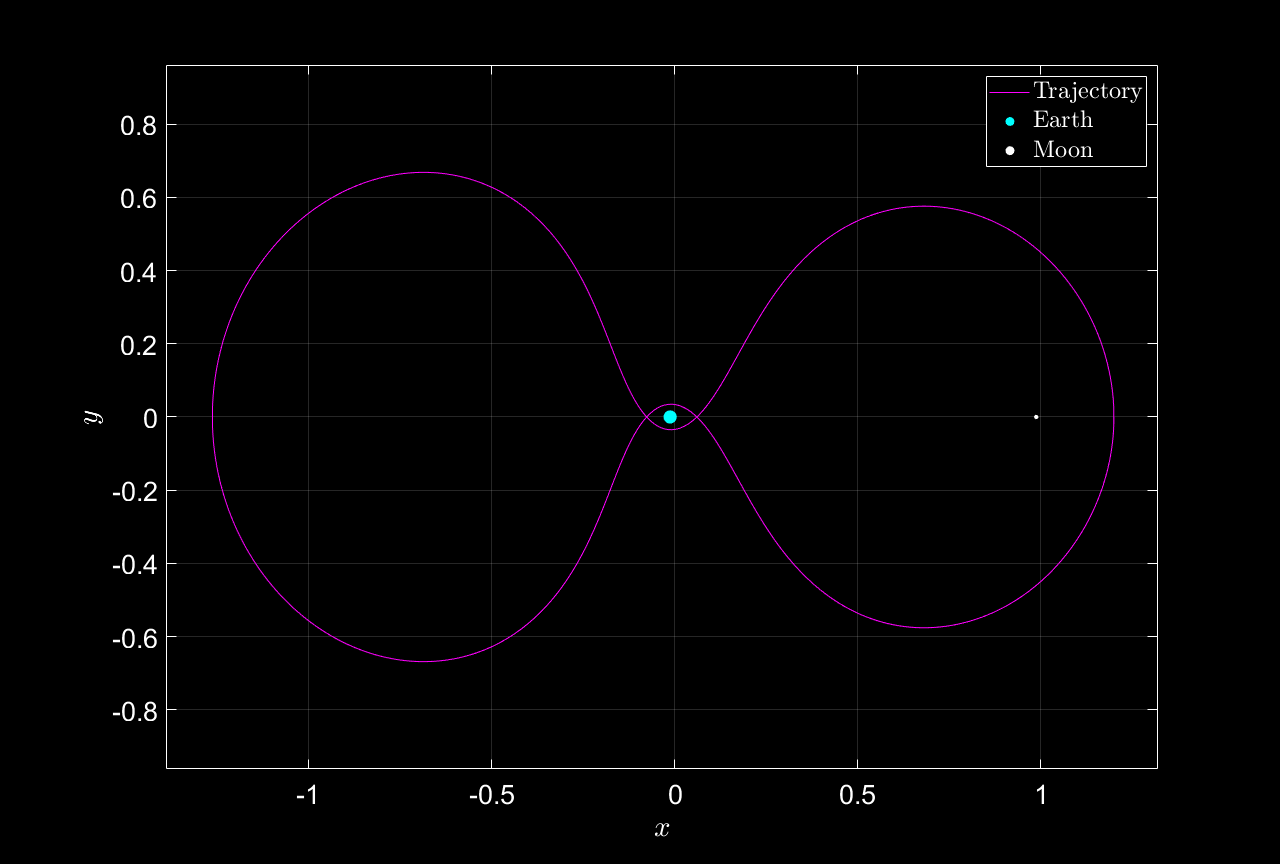
\includegraphics[width=\textwidth]{fig/trajectory1.png}
    \caption{Spacecraft Trajectory about the Earth \& Moon in the Synodic Frame}
    \label{fig1}
\end{figure}

\pagebreak

\begin{figure}[!h]
    \centering
    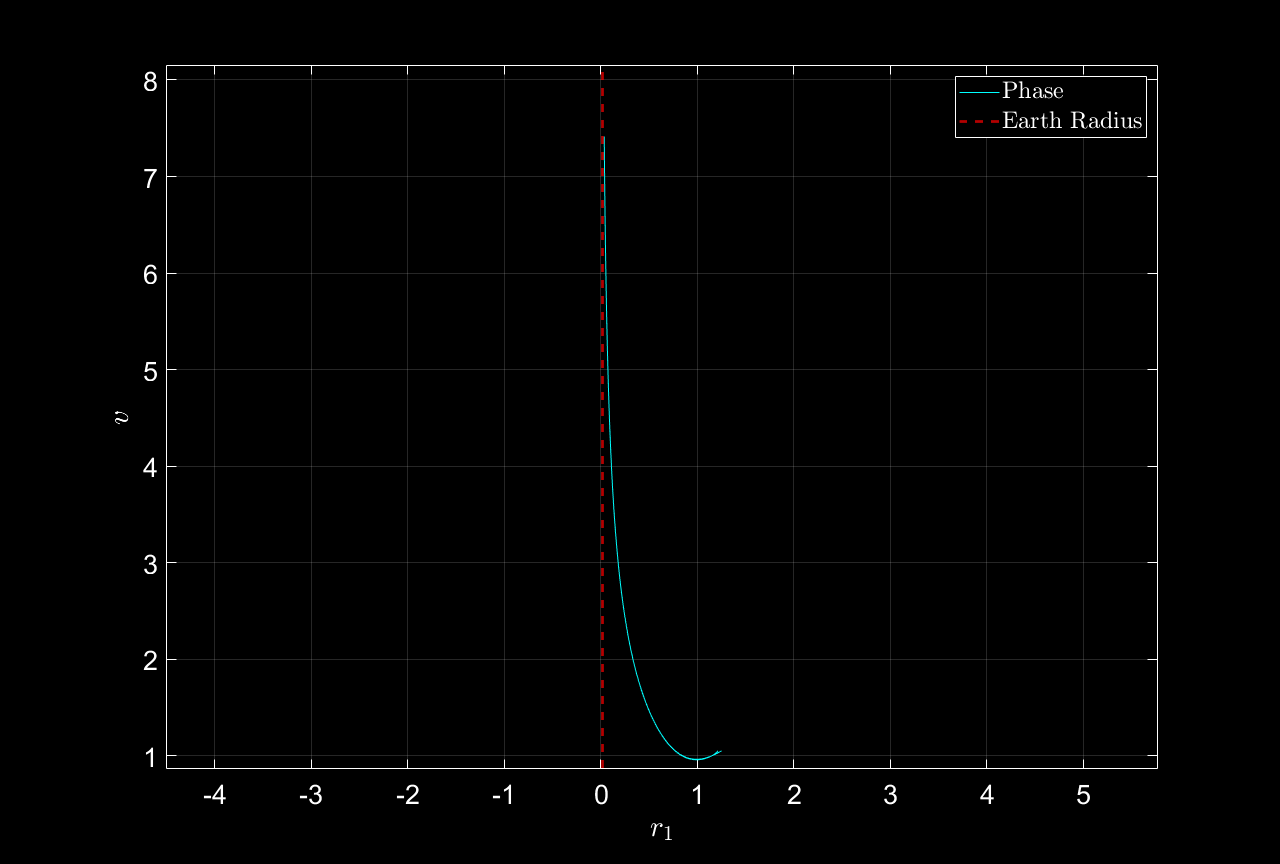
\includegraphics[width=\textwidth]{fig/phase1.png}
    \caption{Phase Space, \textit{Speed vs. Radial Distance from Earth}}
    \label{fig2}
\end{figure}


\begin{table}[h]
    \centering
    \caption{\cw Effects of Increasing the Number of Steps}
    \begin{tabular}{cccc} \toprule
        {$N$} & {$\mathrm{d}t$} & {$r_1$} & {$\mathrm{Test \ Criterion}$} \\ \midrule
        1000  & 0.0150 & 14.7302 & N/A  \\
        2000  & 0.0075  & 212.1128 & 0.9306   \\
        4000  & 0.0038  & 7.0135 & 29.2437   \\ 
        8000  & 0.0019  & 1.2056 & 4.8173   \\
        16000 & $\SI{9.3750E-4}{}$ & 1.1816 & 0.0203 \\
        32000 & $\SI{4.6875e-4}{}$ & 1.1808 & \color{magenta}$\SI{6.3125e-4}{}$ \cw $<$ tol \\ \bottomrule
    \end{tabular}
    \label{tab:table1}
\end{table}



\pagebreak

\subsection*{\underline{Scenario 2:}}

Initial Conditions:
\begin{multicols}{4}
   \begin{itemize}
        \item $x(0)$ = 1.2
        \item $y(0)$ = 0
        \item $v_x(0)$ = 0
        \item $f_d$ = 1
        \item $v_y(0)$ = -1.0493571
  \end{itemize}
\end{multicols}

\textbf{Note}: All quantities are in normalized units.

\vspace{\baselineskip}

These initial conditions are identical to the ones from the Scenario 1, but we set $f_d$ = 1, which corresponds to rockets firing in the retrograde direction with constant thrust through the entire flight. The trajectory will be calculated from $t$ = 0 to 4 normalized time units.

\vspace{\baselineskip}

The results are shown below:

\begin{figure}[h]
  \centering
  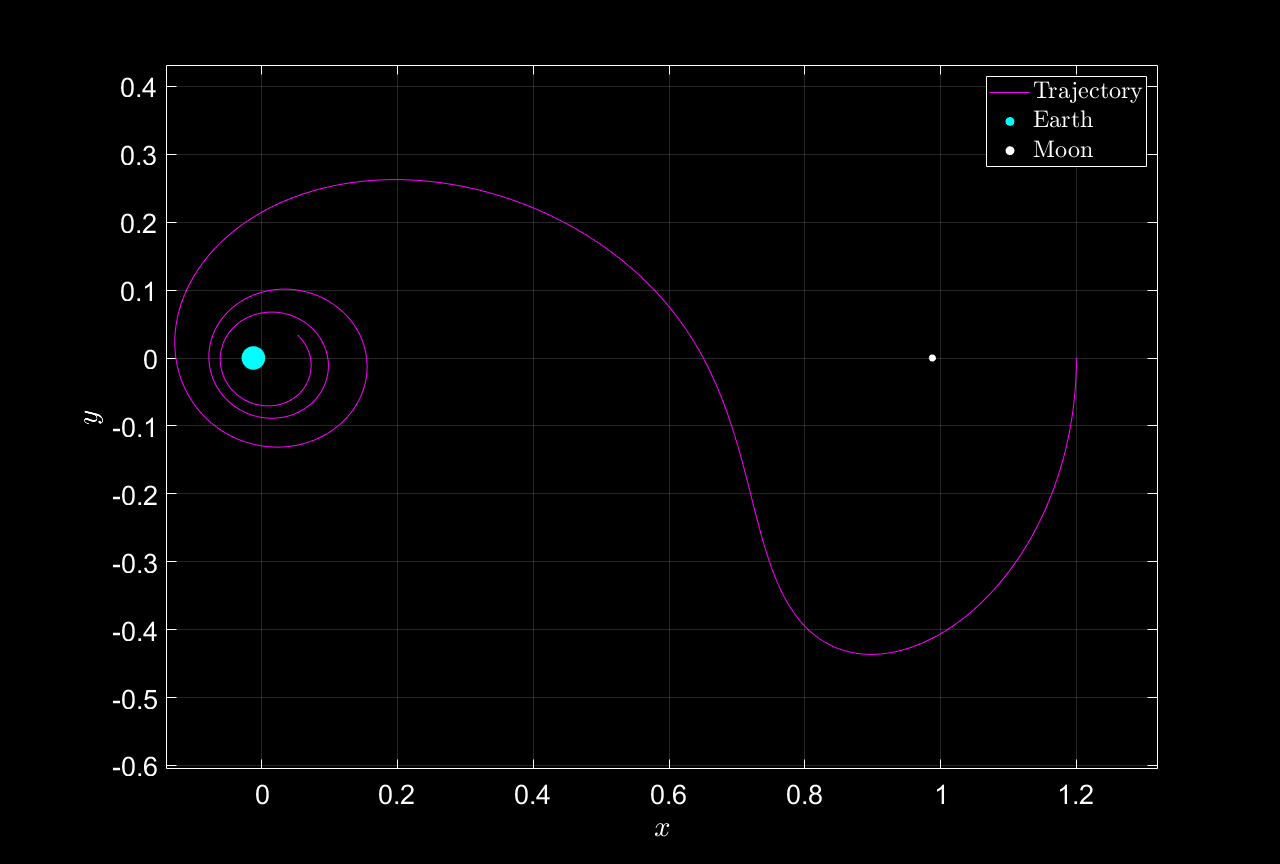
\includegraphics[width=\textwidth]{fig/trajectory2.png}
  \caption{Spacecraft Trajectory about the Earth \& Moon in the Synodic Frame}
  \label{fig3}
\end{figure}

\pagebreak

\begin{figure}[!h]
  \centering
  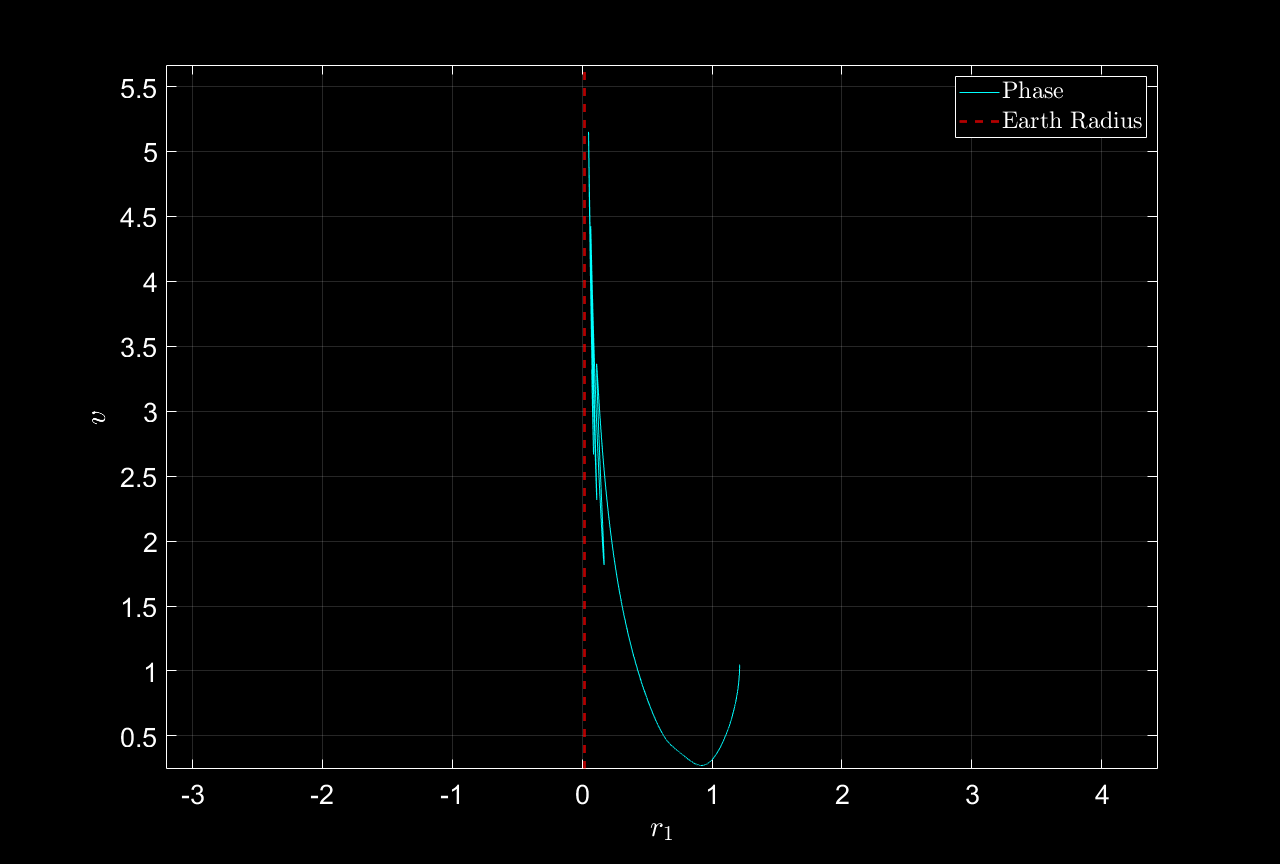
\includegraphics[width=\textwidth]{fig/phase2.png}
  \caption{Phase Space, \textit{Speed vs. Radial Distance from Earth}}
  \label{fig4}
\end{figure}


\begin{table}[h]
  \centering
  \caption{\cw Effects of Increasing the Number of Steps}
  \begin{tabular}{cccc} \toprule
      {$N$} & {$\mathrm{d}t$} & {$r_1$} & {$\mathrm{Test \ Criterion}$} \\ \midrule
      1000  & 0.0040 & 0.0767 & N/A    \\
      2000  & 0.0020 & 0.0748 & 0.0249 \\
      4000  & 0.0010 & 0.0738 & 0.0144 \\
      8000  & 0.0005 & 0.0732 & \color{magenta} 0.0075 \cw $<$ tol \\ \bottomrule
  \end{tabular}
  \label{tab:table2}
\end{table}

\pagebreak

\section{Lagrange Points}

Recall our state vector and derivative of our states:

\begin{equation*}
    \bf{X}
    = \begin{bmatrix}
         x \\
         v_x \\
         y \\
         v_y
       \end{bmatrix},
    \qquad \color{cyan} \dot{\bf{X}} = 
    \begin{bmatrix}
        \dot{x} \\
        \dot{v}_x \\
        \dot{y} \\
        \dot{v}_y
    \end{bmatrix}
    = 
    \begin{bmatrix}
        v_x \\[0.2cm]
        2v_y + x - \ddfrac{\tilde{\mu} \left(x+\mu\right)}{r_1^3} - \ddfrac{\mu \left(x_1-\tilde{\mu}\right)}{r_2^3} - f_d v_x \\[0.2cm]
        v_y \\[0.2cm]
        -2v_x + y - \ddfrac{\tilde{\mu}y}{r_1^3} - \ddfrac{\mu y}{r_2^3} - f_d v_y
    \end{bmatrix}
  \end{equation*}

We can define Lagrange points as locations where:
\begin{equation*}
    \vec{r}(t) = \vec{r}(0) \rightarrow \deriv{\vec{r}}{t} = 0 \rightarrow \deriv{^2\vec{r}}{t^2} = 0
\end{equation*}

\end{document}
